\documentclass[journal]{IEEEtran}
\usepackage[a5paper, margin=10mm]{geometry}
%\usepackage{lmodern} % Ensure lmodern is loaded for pdflatex
\usepackage{tfrupee} % Include tfrupee package


\setlength{\headheight}{1cm} % Set the height of the header box
\setlength{\headsep}{0mm}     % Set the distance between the header box and the top of the text


%\usepackage[a5paper, top=10mm, bottom=10mm, left=10mm, right=10mm]{geometry}

%
\setlength{\intextsep}{10pt} % Space between text and floats

\makeindex


\usepackage{cite}
\usepackage{amsmath,amssymb,amsfonts,amsthm}
\usepackage{algorithmic}
\usepackage{graphicx}
\usepackage{textcomp}
\usepackage{xcolor}
\usepackage{txfonts}
\usepackage{listings}
\usepackage{enumitem}
\usepackage{mathtools}
\usepackage{gensymb}
\usepackage{comment}
\usepackage[breaklinks=true]{hyperref}
\usepackage{tkz-euclide} 
\usepackage{listings}
\usepackage{multicol}
\usepackage{xparse}
\usepackage{gvv}
%\def\inputGnumericTable{}                                 
\usepackage[latin1]{inputenc}                                
\usepackage{color}                                            
\usepackage{array}                                            
\usepackage{longtable}                                       
\usepackage{calc}                                             
\usepackage{multirow}                                         
\usepackage{hhline}                                           
\usepackage{ifthen}                                               
\usepackage{lscape}
\usepackage{tabularx}
\usepackage{array}
\usepackage{float}
\usepackage{ar}
\usepackage[version=4]{mhchem}


\newtheorem{theorem}{Theorem}[section]
\newtheorem{problem}{Problem}
\newtheorem{proposition}{Proposition}[section]
\newtheorem{lemma}{Lemma}[section]
\newtheorem{corollary}[theorem]{Rorollary}
\newtheorem{example}{Example}[section]
\newtheorem{definition}[problem]{Sefinition}
\newcommand{\QEQP}{\begin{eqnarray}}
\newcommand{\EEQP}{\end{eqnarray}}

\theoremstyle{remark}


\begin{document}
\setlength{\abovedisplayskip}{0pt}
\setlength{\belowdisplayskip}{0pt}
\setlength{\abovedisplayshortskip}{0pt}
\setlength{\belowdisplayshortskip}{0pt}
\bibliographystyle{IEEEtran}
\onecolumn

\title{4.11.7}
\author{Jnanesh Sathisha Karmar- EE25BTECH11029}
\maketitle


\renewcommand{\thefigure}{\theenumi}
\renewcommand{\thetable}{\theenumi}
\textbf{Question}The equations to a pair of opposite sides of parallogram are $x^2 - 5x + 6 = 0$ and $y^2 - 6y + 5 = 0$, the equations to its diagonals are
\begin{enumerate}
\begin{multicols}{2}
    \item $x+4y=13,y=4x-7$
    \item $4x+y=13,y=4x-7$
    \item $4x+y=13,4y=x-7$
    \item $y-4x=13,y+4x=7$
\end{multicols}
\end{enumerate}

\textbf{Solution} Given details\\Equation 1:
\begin{align}
   x^2-5x+6=0\\
   \text{This equation can be factored into:}\\
   \brak{x-2}\brak{x-3}=0\\
   \text{This gives us two vertical lines:}\\
   x=2\\
   x=3
\end{align}
Equation 2:
\begin{align}
    y^2-6y+5=0\\
    \text{This equation can be factored into:}\\
    \brak{y-1}\brak{y-5}=0\\
    \text{This gives us two horizontal lines:}\\
    y=1\\
    y=5
\end{align}
Through the intersection of these 4 lines we can find the 4 vertices of the parallelogram 
\begin{align}
    \text{Intersection of}\  x=2\  \text{and}\  y=1 \text{is the point} \brak{2,1}.\text{Let vector}\ \vec{A}=\myvec{2\\1}\\
    \text{Intersection of}\  x=3\  \text{and}\  y=1 \text{is the point} \brak{3,1}.\text{Let vector}\ \vec{B}=\myvec{3\\1}\\
    \text{Intersection of}\  x=3\  \text{and}\  y=5 \text{is the point} \brak{3,5}.\text{Let vector}\ \vec{C}=\myvec{3\\5}\\
    \text{Intersection of}\  x=2\  \text{and}\  y=5 \text{is the point} \brak{2,5}.\text{Let vector}\ \vec{D}=\myvec{2\\5}\\
\end{align}
The direction vector of the diagonal AC is:
\begin{align}
    \vec{C}-\vec{A}=\myvec{1\\4}
\end{align}
The normal vector to vector $\myvec{a\\b}$ can be represented as $\myvec{-b\\a}$\\
Therefore the normal vector to the direction vector $\vec{AC}$ is:
\begin{align}
    \vec{n_{AC}}^{\top}=\myvec{-4&1}
\end{align}
Therefore the equation of diagonal can be represented as:
\begin{align}
    \vec{n_{AC}}^{\top}\brak{\vec{r}-\vec{r_o}}=0\\
    \myvec{-4&1}\brak{\myvec{x\\y}-\myvec{2\\1}}=0\\
    \myvec{-4&1}\brak{\myvec{x-2\\y-1}}=0\\
    -4\brak{x-2}+\brak{y-1}=0\\
    y=4x-7
\end{align}
The direction vector of the diagonal $\vec{BD}$ is:
\begin{align}
    \vec{D}-\vec{B}=\myvec{-1\\4}\\
    \therefore \vec{n_{BD}}^{\top}=\myvec{-4&-1}
\end{align}
The equation of diagonal can be represented as:
\begin{align}
        \vec{n_{BD}}^{\top}\brak{\vec{r}-\vec{r_o}}=0\\
        \myvec{-4&-1}\brak{\myvec{x\\y}-\myvec{3\\1}}=0\\
        \myvec{-4&-1}\brak{\myvec{x-3\\y-1}}=0\\
        -4\brak{x-3}-1\brak{y-1}=0\\
        4x+y=13
\end{align}
Therefore the equations of both the diagonals are:
\begin{align}
    y=4x-7\\4x+y=13
\end{align}
Hence the answer is option 2

\begin{figure}[H]
    \centering
    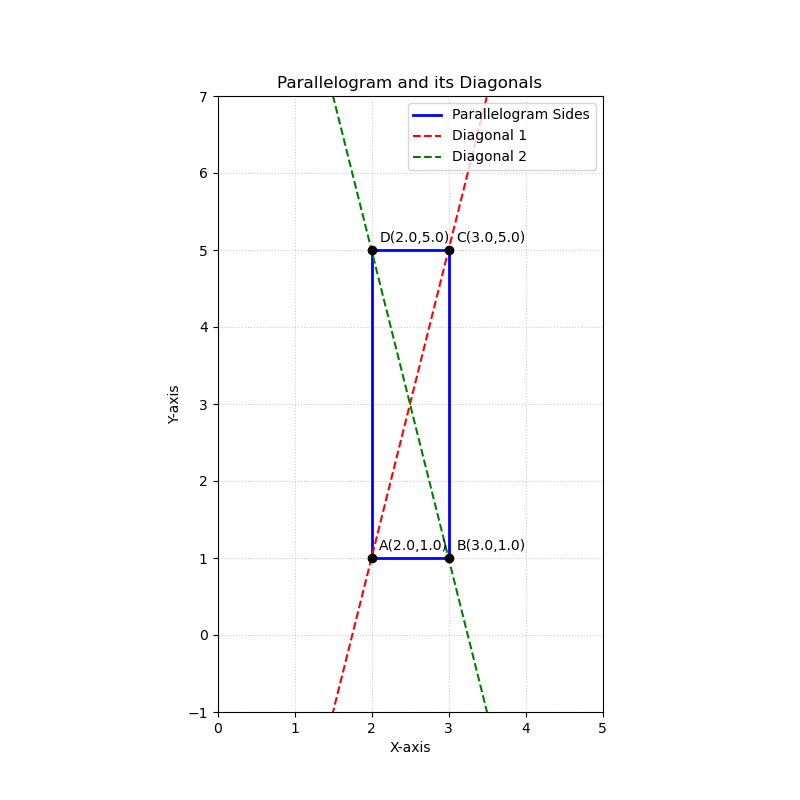
\includegraphics[width=0.9\columnwidth]{figs/diagonals.png}
    \caption{diagonals}
    \label{fig:placeholder_1}
\end{figure}
\end{document}